\documentclass[
	12pt,
	oneside,
	a4paper,
	english,
	brazil
]{abntex2}

\usepackage{lmodern}
\usepackage[T1]{fontenc}
\usepackage[utf8]{inputenc}
\usepackage{indentfirst}
\usepackage{color}
\usepackage{graphicx}
\usepackage{microtype}
\usepackage{amsfonts}
\usepackage{csquotes}

\usepackage{tikz}
\usetikzlibrary{positioning}

\usepackage{caption}

\usepackage[brazilian,hyperpageref]{backref}
\usepackage[alf]{abntex2cite}

\usepackage{macros}

\titulo{Previsão de séries temporais por meio de aprendizado de máquina}
\autor{Guilherme Chichanoski}
\local{Maringá}
\data{2018}
\orientador{Valéria Delisandra Feltrim}
\instituicao{Universidade Estadual de Maringá\\
Centro de Tecnologia --- Departamento de Informática\\
Bacharelado em Ciência da Computação}
\tipotrabalho{Trabalho de Conclusão de Curso}

\preambulo{Trabalho de Conclusão de Curso de Graduação apresentado ao 
Departamento de Informática da Universidade Estadual de Maringá, como requisito 
parcial para obtenção do grau de Bacharel em Ciência da Computação.}

\makeatletter
\hypersetup{
		pdftitle={\@title},
		pdfauthor={\@author},
		pdfsubject={\imprimirpreambulo},
		pdfcreator={LaTeX with abnTeX2},
		pdfkeywords={abnt}{latex}{abntex}{abntex2}{projeto de pesquisa},
		colorlinks=true,	% false: boxed links; true: colored links
		linkcolor=blue,		% color of internal links
		citecolor=blue,		% color of links to bibliography
		filecolor=magenta,	% color of file links
		urlcolor=blue,
		bookmarksdepth=4
}
\makeatother

\setlength{\parindent}{1.3cm}
\setlength{\parskip}{0.2cm}

\begin{document}

\frenchspacing

\imprimircapa{}

\imprimirfolhaderosto{}

\begin{resumo}
    % TODO: Resumo

    \textbf{Palavras-chave}: séries temporais, arima, aprendizado de máquina, 
    redes neurais.
\end{resumo}

\begin{resumo}[Abstract]
    \begin{otherlanguage*}{english}
        % TODO: Abstract

        \textbf{Keywords}: séries temporais, arima, aprendizado de máquina, 
        redes neurais.
    \end{otherlanguage*}
\end{resumo}

\textual{}

\pdfbookmark[0]{\contentsname}{toc}
\tableofcontents*
\cleardoublepage{}

\chapter{Introdução}

Segundo \citeonline{wiley} prever é a tarefa de predizer valores futuros ou 
eventos, é de grande importância para diversos setores incluindo governos e 
industrias, podendo ser parte crucial na tomada de decisão fica evidente a 
necessidade de se realizar boas previsões. No entanto, autores e organizações 
renomadas já realizaram previsões que se demonstraram erradas, como exemplo 
podemos citar The New York Times que previu em 1966 que em 2000 existiriam 
somente 220.000 computadores nos Estados Unidos.

Ainda conforme \citeonline{wiley} as previsões são classificadas como sendo de 
curto, médio e longo prazo. Quando denominada de curto é previsto somente poucas 
observações a frente, podendo ser contados em horas, dias ou semanas. Já 
previsões de médio prazo podem se estender por algumas observações no futuro com 
os passos podendo ser dados em meses ou anos, enquanto períodos maiores serão 
chamados de longo prazo. Ainda segundo o autor, predições de médio e longo prazo 
são mais difíceis e suscetíveis a fatores externos.

Em \citeonline{giebel2011state} o autor realiza a predição da geração de energia 
eólica, a produção é dada em função da capacidade na região instalada, o vento, 
no entanto, é um elemento volátil e sendo assim existirá momentos quais o uso de 
outras fontes será necessária, no entanto, é preciso ter certo conhecimento 
prévio, pois, o ligamento de uma usina como aquelas movidas a gasóleo podem 
levar até duas horas. Logo prever duas horas a frente pode ser crucial para 
garantir o abastecimento de energia a uma região, podendo impactar no cotidiano 
e economia de uma população.

Empresas se beneficiam de diversas formas ao aplicar previsões no seu processo 
de tomada de decisão, em especial, durante tarefa de manutenção do estoque com 
vista em maximizar a satisfação dos clientes e obtenção de lucros, ao suprir a 
demanda por seus produtos, impedindo que clientes se frustem em caso de 
desabastecimento, e impedir excedentes não vendidos. Considerando esta 
necessidade, se propôs com base nos dados de vendas elaborar modelos que sejam 
capazes de prever demandas futuras, fornecendo dados para corroborar na compra e 
manutenção dos estoques, a informação se organizará na forma de uma série 
temporal.

% FIXME: Tá esquisito
As séries temporais, segundo \citeonline{wiley} são compostas de observações 
sequenciais ao longo do tempo, como exemplo, podemos observar a série na 
\autoref{serie0}, que foi gerada utilizando um processo de caminhada aleatória.  
Sendo essas observações separadas unicamente pelo tempo pode-se obter os dados 
em diferentes intervalos, como observações diárias, semanais ou ainda anuais.  
Conforme \citeonline{ehlers} devido a caraterística estocástica, uma observação 
é dada em função da anterior, é possível elaborar modelos que descrevem o 
comportamento e permitem a prever os valores futuros.

\begin{figure}[ht]
    \centering
    \caption{Série gerada para exemplo}\label{serie0}
    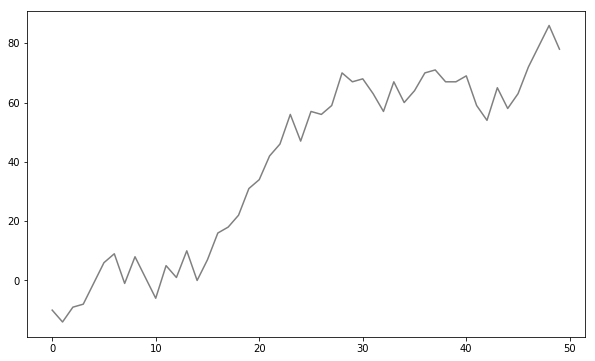
\includegraphics[width=.6\linewidth]{images/serie_exemplo.png}
    \source{Elaborado pelo autor}
\end{figure}

% TODO: Introduzir modelos ARIMA com exemplos de artigos

Em contrapartida, técnicas de aprendizado de máquinas estão se tornando cada vez 
mais notórias pelos bons resultados que oferecem. \citeonline{artigoEx3} aplicou 
métodos de aprendizado de máquina possibilitando a previsão com bons resultados.  
Pelo fato dos modelos estatísticos serem considerados quase um padrão para 
predições, é comum que trabalhos como \citeonline{artigoEx4} compare os 
resultados obtidos a partir de aprendizado de máquina com modelos de abordagem 
estatísticas. Para modelos de aprendizado se destaca aqueles com uso de redes 
neurais artificiais por serem capazes de obter bons resultados conforme 
analisado por \citeonline{zhang}, o autor ainda apresenta outros exemplos quais 
os autores obtiveram resultados superiores ao método estatístico.

No \autoref{chap:fundTeor}, será apresentada a definição da atividade de 
previsão seguido dos principais métodos de previsão de séries temporais 
empregadas, sendo o primeiro, ARIMA, com abordagem estatística e o segundo 
usando com base em métodos de aprendizado de máquina, sendo especificamente 
descrito as redes neurais artificiais de múltiplas camadas. Após apresentado os 
métodos, no \autoref{chap:desenv} conforme objetivos estabelecidos serão 
propostos dois modelos, um utilizando o modelo probabilístico e o outro tendo 
base o modelo neural. Com base nos modelos obtidos serão apresentados os 
resultados no \autoref{chap:result} e finalizando com a discussão das métricas 
obtidas no \autoref{chap:concl}.

\chapter{Fundamentação teórica}\label{chap:fundTeor}

\section{Previsão}
Segundo \citeonline{wiley} podemos separar o processo de previsão em diversas 
atividades, colocadas e detalhadas a seguir:

\begin{itemize}
	\item Definição do problema\\
		Envolve definir e entender a tarefa de previsão a ser realizada,
        considerando o prazo a ser previsto e definindo os dados necessários.
	\item Coleta dos dados\\
		Conforme definido na etapa anterior ocorrerá nessa atividade a coleta
		dos dados.
	\item Análise dos dados\\
		Atividade de alta importância para a seleção do modelo mais adequado,
        nessa etapa é utilizada de observações gráficas e extração de 
        características para identificar padrões que corroborem na escolha dos 
        parâmetros. Ainda ocorrerá a identificação de observações problemáticas 
        e corrigidas.
	\item Seleção e verificação do modelo\\
        Conforme analisado será selecionado o modelo, analisando também o 
        comportamento com os dados fornecidos. Como método de verificação será 
        utilizado métricas que permitam comparar com outros modelos.
	\item Avaliação do modelo\\
        Etapa para avaliar como o modelo se comportará com novos dados, 
        normalmente é realizado com observações extraídas dos dados utilizados 
        nas etapas anteriores, porem a parte separada terá somente esta 
        finalidade.
	\item Publicação do modelo\\
        Com o modelo devidamente selecionado e avaliado é instalado em ambiente 
        de produção, tendo que observar as alterações necessárias para que novos 
        dados sejam inseridos corretamente.
    \item Monitoramento do desempenho do modelo\\
        Deve-se continuamente avaliar como o modelo aplicado se comporta em 
        relação ao ambiente, já que o ambiente é algo volátil.
\end{itemize}

Vale-se notar que após a tarefa de avaliação se essa resultar em um valor 
insatisfatório deve-se retornar a fase anterior e refeita a avaliação até que um 
modelo que obedeça às especificações seja encontrado.

\section{Séries temporais}

Como já colocado anteriormente, séries temporais são observações sucessivas ao 
longo do tempo. Retomamos ainda que essas séries se caracterizam pelo fato de 
suas observações serem dependentes das observações anteriores. Demonstram 
características como tendência e sazonalidade, sendo que a primeira capaz de 
conferir a série um comportamento lento que pode levar a observações futuras com 
valores menores ou maiores e a segunda característica impõe a ela padrão que 
apresente ciclos, podendo ser estes semanais, mensais, anuais ou um período 
qualquer de tempo.

Uma série é descrita matematicamente pelo conjunto $\{X(t): t \in T\}$, podendo 
ser $t$ um tempo contínuo ou discreto, sendo continuo quando se possui as 
observações de todo $t$ em $T$, sendo este dado como $T \subseteq 
\mathbb{R}^{+}$ e discreto quando entre uma observação e outra existe um 
intervalo igual de tempo, normalmente dado na forma de uma sequência, $T = \{1, 
2, \ldots, n\}$, sendo $n$ o número de leituras.

Segundo \citeonline{ehlers} uma série temporal classicamente é decomposta 
seguindo a \autoref{eq:timeseries}, sendo $t$ usado para denotar o tempo, $T$ 
nos fornece a tendência, $C$ a sazonalidade, já $R$ é a componente aleatória e 
caracterizada por possuir média zero, denotada como ruído branco.

\begin{equation}
	\label{eq:timeseries}
	X_t = T_t + C_t + R_t
\end{equation}

\subsection{Série estacionária}

Um conceito importante em séries é o caráter estacionário, e segundo 
\citeonline{ehlers} definimos uma série estritamente estacionária por possuir a 
distribuição de probabilidade conjunta de $X(t_1), \ldots, X(t_k)$ igual de 
$X(t_1 + \tau), \ldots, X(t_k + \tau)$.

Ainda segundo \citeonline{ehlers} a definição dada é dificilmente aplicada, 
então usamos a definição de fracamente estacionaria para definir se é 
estacionária, definindo então com base no critério de possuir função média 
constante.

Em outras palavras, o deslocamento da origem do tempo $t$ por uma quantidade 
$\tau$ não exerce efeito na distribuição conjunta da série, assim o valor 
esperado para a série em determinado não será dada em função do tempo.

A \autoref{fig:co2diff} é um exemplo de série estacionária encontrada utilizando 
o processo de diferenciação que será descrita na \autoref{sec:diff}.

\subsection{Tendência}

Segundo \citeonline{ehlers} não existe uma definição precisa de tendência, mas 
normalmente é associado ao comportamento de mudança das observações em período 
de longo prazo. Uma série com tendência pode ser descrita como uma função 
apresentada na \autoref{eq:tendencia}, $\alpha$ e $\beta{}$ coeficientes e 
$\epsilon{}_t$ o erro. Sendo que $\beta{}$ define a taxa de crescimento da 
série, assim podemos entender $\beta$ da forma $\beta = x_t - x_{t-1}$.

\begin{equation}
	\label{eq:tendencia}
	X_t = \alpha + \beta{}t + \epsilon{}_t
\end{equation}

Este entendimento de série com tendencia segundo \citeonline{ehlers} permite 
encontrar uma função polinomial que represente a série, no caso esta função 
teria a forma da \autoref{eq:tendenciaSerie}.

\begin{equation}
    \label{eq:tendenciaSerie}
    X_t = \beta_0 + \beta_1t + \beta_2t^2 + \cdots + \beta_{p}t^p + \epsilon_t
\end{equation}

Para exemplificar uma série temporal real que apresente tendência e sazonalidade 
podemos apresentar o gráfico na \autoref{fig:co2}, este apresenta a mudança na 
concentração de $CO_2$ na atmosfera, no caso esta é uma série de um dado natural 
e é fácil notar o comportamento tendencioso e sua sazonalidade, que no caso é 
anual.

\begin{figure}
    \centering
    \caption{Leituras de $CO_2$ na atmosfera.}\label{fig:co2}
    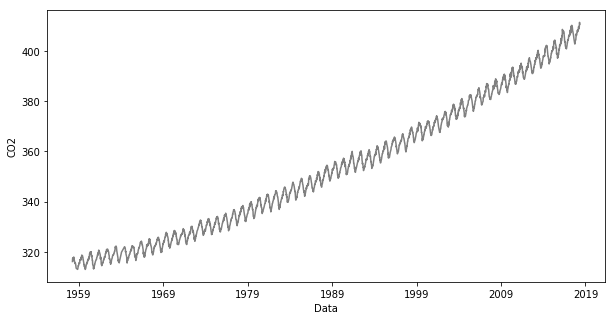
\includegraphics[width=.6\linewidth]{images/co2.png}
    \source{\citeonline{co2data}}
\end{figure}

\subsubsection{Filtros}

Em algumas séries a tendência pode não estar evidente devido à flutuações, 
nesses casos é comum a aplicação de um filtro que tem como objetivo obter uma 
série suavizada que possibilite observar a tendência, esse filtro é da forma da 
\autoref{eq:filtro}\cite{ehlers}.

\begin{equation}
    \label{eq:filtro}
    y_t = \sum_{j = -q}^{s}{a_{j}x_{t+j}}
\end{equation}

Na \autoref{eq:filtro} $a_j$ é um coeficiente a ser aplicada a cada termo da 
soma de forma a aplicar um peso a este, sendo observado que $\sum{a_j} = 1$.
Podemos obter no caso mais simples $a_j = \frac{1}{2q + 1}$ e teremos $y_j$ 
conforme a \autoref{eq:yjfiltro}.

\begin{equation}
    \label{eq:yjfiltro}
    y_t = \frac{1}{2q + 1}\sum_{j=-q}^{q}{x_{t+j}}
\end{equation}

A \autoref{eq:yjfiltro} é conhecida por fornecer o cálculo das médias móveis. A 
aplicação do filtro de médias móveis na série das leituras de $CO_2$ resulta na 
\autoref{fig:co2filtrado}, que demonstra de forma independente a tendência da 
série após removido a sazonalidade.

\begin{figure}
    \centering
    \caption{Leituras de $CO_2$ filtrada utilizando médias móveis com $q$ igual a 
    $52$, devido à sazonalidade ser anual, ou seja, $52$ 
    semanas.}\label{fig:co2filtrado}
    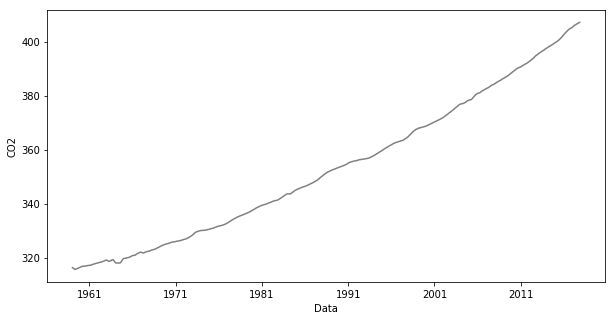
\includegraphics[width=.6\linewidth]{images/co2_filtered.png}
    \source{Elaborado pelo próprio autor a partir de \citeonline{co2data}}
\end{figure}

\subsubsection{Diferenciação}\label{sec:diff}

Outra tarefa a ser observada em relação ao entendimento de tendência é a forma 
qual é removida, para sua remoção o método mais simples para tal é fazer a 
subtração do elemento com o seu antecessor, da forma como descrito na 
\autoref{eq:diferenciacao}, normalmente uma única diferenciação é suficiente 
porem em séries com componente sazonal podem vir a ser necessárias mais de uma 
em um \textit{lag} diferente.

\begin{equation}
    \label{eq:diferenciacao}
    y_t = x_t - x_{t-1}
\end{equation}

Para dar um exemplo de diferenciação volto a série das leituras do $CO_2$ e agora 
realizando uma diferenciação, o resultado é visto na \autoref{fig:co2diff}, 
especificamente neste exemplo percebemos que a série se aproximou de uma série 
com função média constante, dando evidência a componente de sazonal.

\begin{figure}
    \centering
    \caption{Série da leitura do $CO_2$ na atmosfera com uma 
    diferenciação}\label{fig:co2diff}
    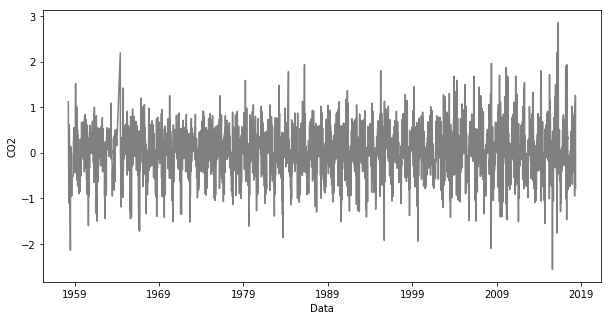
\includegraphics[width=.6\linewidth]{images/co2_diff.png}
    \source{Elaborado pelo autor a partir de \citeonline{co2data}}
\end{figure}

%\subsection{Sazonalidade}
%
%Conforme definido por \citeonline{ehlers} sazonalidade caracteriza repetições de 
%comportamento de uma série em um período $s$ de tempo. Podemos expressar uma 
%série sazonal usando a \autoref{eq:sazonal}

% TODO: Falta um tanto aqui

\section{Modelos probabilísticos}

Como já disposto, as séries temporais podem ser previstas utilizando de modelos 
estatísticos, isso segundo \citeonline{ehlers} ocorre devido ao seu caráter 
estocástico por conta de cada observação possuir correlação com as observações 
anteriores.

O modelo comumente utilizado para essa tarefa é o ARIMA, descrito por 
\citeonline{box}, caracteriza a série em três parâmetros $(p,d,q)$, sendo cada 
um associado a um processo, sendo $p$ associado a processos auto-regressivos, 
$r$ a processos integrativos e $q$ a de médias móveis.

\subsection{Função de autocorrelação}\label{sec:corre}

Durante a parametrização precisaremos identificar o comportamento da série, uma 
ferramenta para isso é a função de autocorrelação descrita em 
\autoref{eq:autocorrelacao} para a defasagem $k$.

\begin{equation}
    \label{eq:autocorrelacao}
    r_k = \frac{\sum_{t=1}^{n-k}{(x_t - \overline{x})(x_{t+k} - 
    \overline{x})}}{\sum_{t=1}^{n}{(x_t - \overline{x})^2}}
\end{equation}

Segundo \citeonline{ehlers} a função de autocorrelação quando plotada para os 
$k$-ésimos primeiros coeficientes é chamado de correlograma e este é uma 
ferramenta importante para as análises, como exemplo pode ser visto a 
\autoref{fig:correlogramaCo2} na qual é disposto as 25 primeiras defasagens das 
leituras de concentração de $CO_2$ na atmosfera, ainda segundo 
\citeonline{ehlers} temos de definir ao correlograma o seu intervalo de 
confiança, com o qual podemos considerar tudo que esteja acima desse como uma 
correlação que deve ser analisada e abaixo desse limite será desconsiderada, 
assim se todos as correlações estarem abaixo desse limite podemos considerar a 
série como um ruído branco, para encontrar esse intervalo \citeonline{ehlers} 
recomenda utilizar a seguinte equação $\pm{}1,96/\sqrt{n}$, sendo $n$ o número 
de observações da série.

\begin{figure}
    \centering
    \caption{Gráfico da função de autocorrelação das leituras de 
    $CO_2$}\label{fig:correlogramaCo2}
    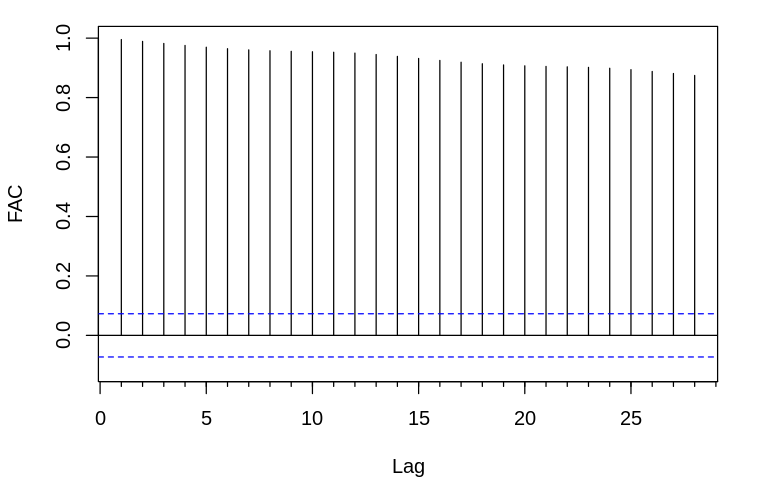
\includegraphics[width=.6\linewidth]{images/acf_co2.png}
    \source{Elaborado pelo autor a partir de \citeonline{co2data}}
\end{figure}

Pela \autoref{fig:correlogramaCo2} podemos concluir que as leituras do $CO_2$ 
apresentam uma tendência, e ainda por apresentar todos valores positivos podemos 
afirmar que crescerá ao longo do tempo. Como a série possui tendência temos de 
fazer uma diferenciação, como disposto na \autoref{sec:diff}, para remoção dessa 
componente, vemos a série após essa diferenciação na \autoref{fig:co2diff} e o 
correlograma após a diferenciação pode ser visto na \autoref{fig:acfco2diff}, 
nesse novo gráfico é percebido que a componente da tendência foi realmente 
removida após uma diferenciação, tornando visível a componente sazonal, vemos 
isso pela alternância das correlações observadas no correlograma.

\begin{figure}
    \centering
    \caption{Gráfico de função de autocorrelação da diferenciação da série de 
    $CO_2$}\label{fig:acfco2diff}
    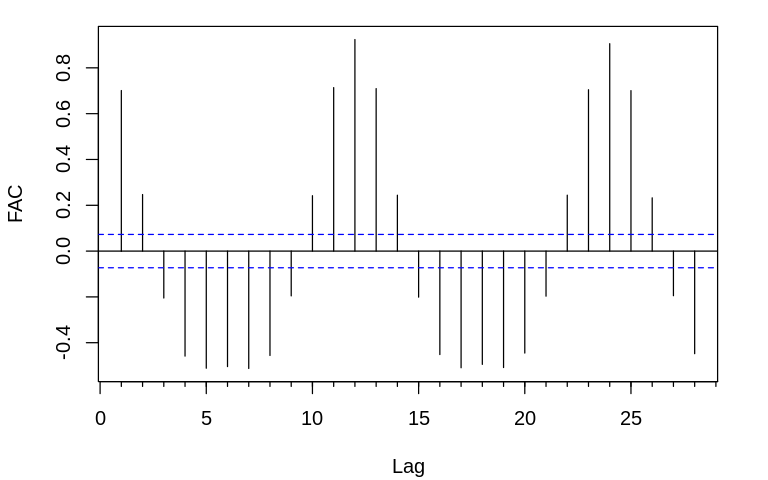
\includegraphics[width=.6\linewidth]{images/acf_co2_diff.png}
    \source{Elaborado pelo autor a partir de \citeonline{co2data}}
\end{figure}

% TODO: Citar as seções nas quais o correlograma é apresentada em outros 
%cenários

\subsection{ARIMA}



\section{Aprendizado de Máquina}

Segundo \citeonline{machineLearning} aprendizado de máquina é descrito como a 
habilidade de algorítimos reconhecer padrões em um conjunto de dados.

Esses padrões a serem encontrados permitirão que tarefas como as seguintes seja, 
realizadas:
\begin{itemize}
    \item Classificação\\
        É a tarefa de mapear uma entrada a uma \textit{tag}, como no exemplo na 
        classificação dos números, apresentada no início da seção. Podemos 
        encontrar ainda exemplos do uso de aprendizado de máquina para 
        classificação em diversos outros trabalhos, como 
        \citeonline{artigoClassificacao} que utilizou redes neurais artificiais 
        para realizar a classificação de imagens.
    \item Regressão\\
        Já a tarefa de regressão é aplicada quando precisamos mapear um conjunto 
        de valores a uma saída em $ \mathbb{R} $, \citeonline{regressao} 
        utilizou redes neurais artificiais para encontrar um modelo que 
        permitisse a previsão da demanda de uso de energia elétrica, mapeando o 
        carga atual e informações climáticas a carga futura.
\end{itemize}

Um exemplo de uso de aprendizado de máquina é a identificação de caracteres 
numéricos escritos a mão, esse exemplo é apresentado por 
\citeonline{machineLearning} e o descreve como um problema de classificação no 
qual uma imagem de dimensões $28 \times 28$ pixeis é dada como entrada em um 
algorítimo e este deve atribuir uma classificação que descreve qual o número que 
a figura representa, um conjunto de exemplo dessas imagens pode ser visto na 
\autoref{fig:numeroClassi}.

\begin{figure}
    \centering
    \caption{Exemplo de entrada para o algorítimo de 
    classificação}\label{fig:numeroClassi}
    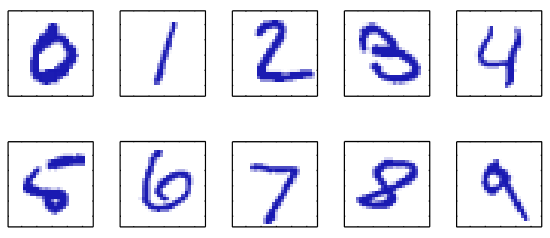
\includegraphics[width=.6\linewidth]{images/numeroClassificacao.png}
    \source{\citeonline{machineLearning}}
\end{figure}

\subsection{Redes Neurais artificiais}

Segundo \citeonline{haykin} a pesquisa em redes neurais artificiais é motivada 
pelo entendimento que o cérebro humano realiza o processamento de uma forma 
completamente diferente dos computadores convencionais. Essa forma de realizar o 
processamento realizado pelo cérebro é altamente complexa, não linear e 
altamente paralela. A unidade de processamento e organização básica de um 
cérebro são os neurônios, o autor ainda lhe confere superior capacidade na 
realização de tarefas como reconhecimento de padrões do que os computadores 
digitais.

Os animais já nascem com o cérebro possuindo certa estruturas que estes vão 
precisar durante sua vida, porem este é concebido ainda de maneira muito 
plastica, ou seja, possuindo ainda a capacidade de na fase de aprendizado ser 
capaz de se adaptar ao contexto em que vai se desenvolver. Este mesmo conceito 
de plasticidade também será utilizado para a modelagem de redes neurais 
artificiais~\cite{haykin}.

\subsubsection{\textit{Perceptron}}

Como já colocado, as redes neurais possuem o neurônio como elemento de 
processamento, este em redes artificiais associamos ao \textit{perceptron}, 
descrito primeiramente por Rosenblatt em 1958, e tem sua função definida em 
\autoref{eq:perceptron} sendo dado como a soma ponderada por $w_i$ das entradas, 
$x_i$.

\begin{equation}
    \label{eq:perceptron}
    v = \sum_{i=1}^{m}{w_i + b}
\end{equation}

% TODO: Algorítimo
% TODO: MLP
% TODO: Back Propaggation
% TODO: Descida de Gradiente
% TODO: - Adam

\subsubsection{MLP}

\subsubsection{Adam}

\chapter{Desenvolvimento}\label{chap:desev}

Para demonstrar e avaliar a capacidade de os métodos de previsão apresentados 
neste trabalho, foi selecionada uma série temporal qual consta as vendas diárias 
de uma rede de farmácias germânica, os dados foram obtidos 
\textit{online}\footnote{Kaggle 
\url{https://www.kaggle.com/c/rossmann-store-sales}}.

Foram realizadas algumas etapas de pré processamento dos dados antes de obtermos 
a série temporal efetivamente utilizada para a previsão.  Primeiramente foi 
necessária a seleção de uma loja aleatoriamente, já que o conjunto de dados 
obtidos nos traz dados das diversas lojas que compõe a rede.  Foi selecionada 
então de forma aleatória a loja de ID 67. Após foi então obtida uma série 
temporal multivariada, entretanto, a proposta deste trabalho é a avaliação de 
previsões em séries uni variadas, ou seja, embora o conjunto de entrada possua 
mais informação que aquelas que serão utilizadas para previsão, estas serão 
descartadas. Logo a série será composta somente da quantidade diária de vendas 
realizadas. O gráfico que apresenta a série a ser encontrado o modelo é vista na 
\autoref{fig:serieRossman}.

\begin{figure}[ht]
    \centering
    \caption{Gráfico de observações das vendas diárias}\label{fig:serieRossman}
    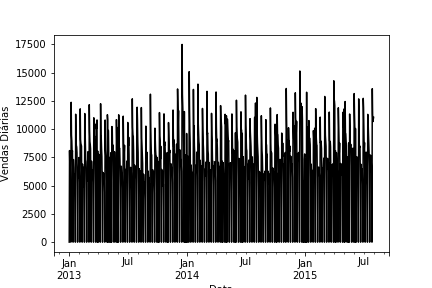
\includegraphics[width=.6\textwidth]{images/graficoRossman.png}
    \source{Elaborado pelo autor}
\end{figure}

\begin{figure}[ht]
    \centering
    \caption{Gráfico contendo 3 semanas de observações para visualização do 
    comportamento semanal da série}\label{fig:serieRossmanSemana}
    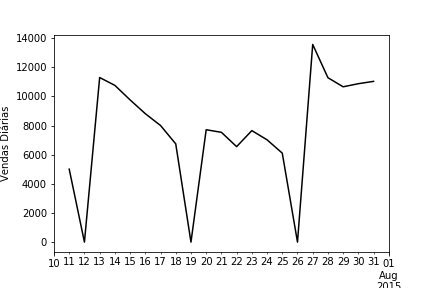
\includegraphics[width=.6\textwidth]{images/graficoRossmanSemana.png}
    \source{Elaborado pelo autor}
\end{figure}

Observamos na \autoref{fig:serieRossman} a existência de valores que podem ser 
descritas como \textit{outliers}, isto é, são leituras que estão fora do padrão 
esperado, isso ocorre devido às observações serem diárias e a rede de farmácia 
não possuir expediente aos domingos, pode ser visto de forma mais clara na 
\autoref{fig:serieRossmanSemana}, nesses dias as leituras aparecerão zeradas e 
assim gerando uma série que embora com maior número de observações possuirá 
instabilidade, que aumenta consideravelmente a complexidade do modelo, para 
evitar esse problema foi realizada a conversão para observações semanais, 
somando a quantidade de vendas realizada em uma semana em um único valor, essa 
nova série é apresentada na \autoref{fig:serieRossmanSemanal}.

\begin{figure}[ht]
    \centering
    \caption{Gráfico de observações semanais de 
    vendas}\label{fig:serieRossmanSemanal}
    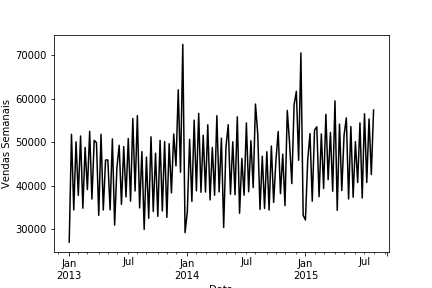
\includegraphics[width=.6\textwidth]{images/graficoRossmanSemanal.png}
    \source{Elaborado pelo autor}
\end{figure}

\section{Análise da série}

Para continuarmos com a parametrização dos modelos que serão avaliados temos de 
ter uma boa compreensão do comportamento da série, para isso são aplicadas 
algumas ferramentas apresentados como o correlograma descrito na 
\autoref{sec:corre}.

Em primeira analise observamos na \autoref{fig:serieRossmanSemanal} que em dois 
momentos a série apresenta máximos locais, observado de forma detalhada na 
\autoref{fig:rossmanFimAno}.

\begin{figure}
    \centering
    \caption{Gráfico do comportamento da série no fim do 
    ano}\label{fig:rossmanFimAno}
    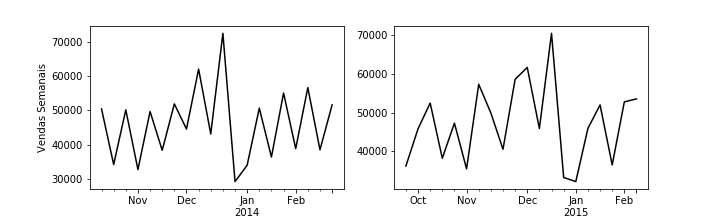
\includegraphics[width=.8\textwidth]{images/graficoRossmanFimAno.png}
    \source{Elaborado pelo autor}
\end{figure}

O conjunto de dados utilizado, ainda nos trás outras informações, como se houve 
promoção naquele dia ou se foi feriado. Se considerarmos essas informações 
podemos compreender algumas flutuações que ocorrem na série, por exemplo se 
observarmos a \autoref{fig:rossmanPromo} vemos que os maiores volumes de venda 
tendem a ocorrer nos dias de promoção.

% TODO: Gerar essa imagem
\begin{figure}
    \centering
    \caption{Observações marcados conforme ocorrência de promoções}
    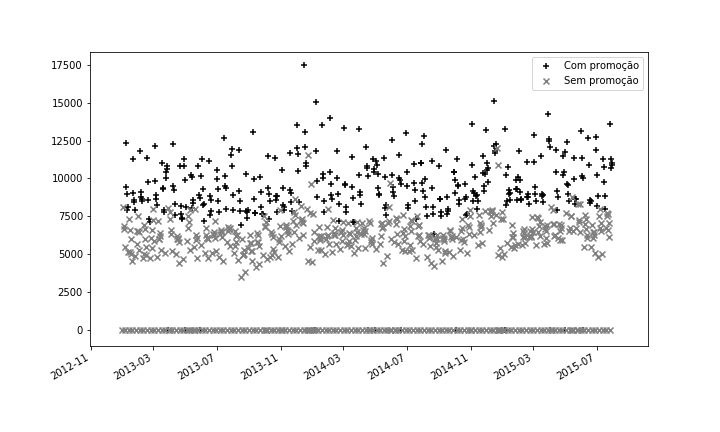
\includegraphics[width=.7\textwidth]{images/graficoRossmanPromo.png}
    \source{Elaborado pelo autor}
\end{figure}

Aplicando então a função de autocorrelação apresentada anteriormente obteremos 
informações para a parametrização do modelo, utilizando a série com frequência 
semanal apresentado na \autoref{fig:serieRossmanSemanal} teremos a seguinte 
\autoref{fig:acfRossmanSemanl}.

% \begin{figure}
%     \centering
%     \caption{Função de Autocorrelação aplicada a série}
%     \includegraphics[width=.7\textwidth]{images/graficoAcfSemanal.png}
%     \source{Elaborado pelo autor}
% \end{figure}

\section{Aprendizado de máquina}

Diferentemente do ARIMA, redes neurais artificiais não foram elaboradas com a 
visão na aplicação de previsão de redes neurais, na verdade seu uso é muito mais 
abrangente que este, no entanto, se considerarmos o problema de previsão de 
redes neurais como um problema de regressão poderemos modelar a rede neural para 
que a saída desta seja a próxima observação da série.

A entrada da rede neural foi estabelecida como duas observações no passado, 
porem poderia ser utilizado mais, mas para manter o modelo parcimonioso foi 
mantido assim.

Na etapa de escolha dos parâmetros foi utilizado busca em grade com validação 
cruzada, com \textit{fold} de tamanho cinco. Os parâmetros testados estão 
apresentas na \autoref{tab:grid}, para validação do modelo foi calculado o MAPE 
e então selecionado aquele que melhor representou a série.

\begin{table}
    \centering
    \caption{Parâmetros testados na busca em grade}\label{tab:grid}
    \begin{tabular}{ l r }
        \toprule
        Parâmetros                      & Valores testados\\
        \midrule
        Número de camadas escondidas    & [1, 2, 3, 4]\\
        Número de neurônios por camadas & [2, 4, \ldots, 100]\\
        Função de ativação              & [relu, tanh]\\
        Número de épocas                & [500, 1000, 1500]\\
        Otimizador                      & [adam, sgd]\\
        \bottomrule
    \end{tabular}
    \source{Elaborado pelo autor}
\end{table}

Após execução, o resultado da busca em grade retornou que a melhor escolha a 
utilização de somente uma camada escondida com 12 neurônios, alem disso a função 
de ativação ficou estabelecida como a relu, com otimização usando adam. A 
arquitetura da rede neural resultante é demonstrada na \autoref{fig:redeNeural}. 

\begin{figure}
    \centering
    \caption{Representação gráfica da rede neural artificial utilizada para 
    avaliação}\label{fig:redeNeural}
    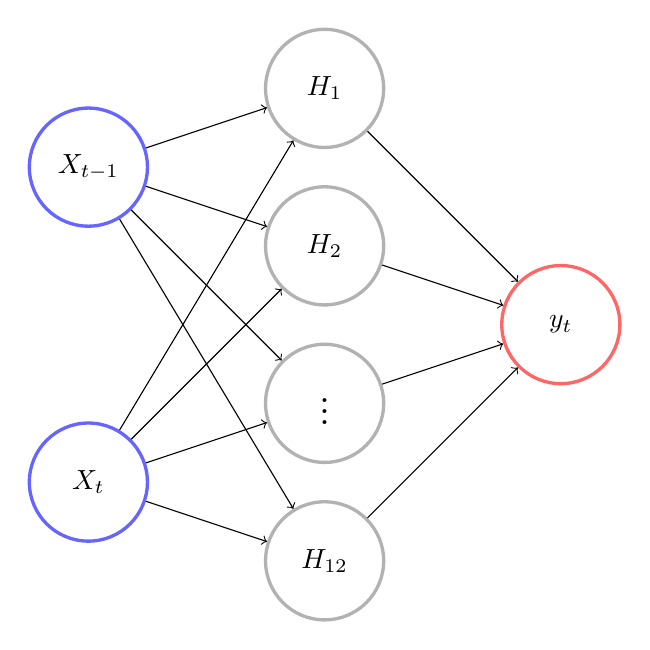
\begin{tikzpicture}[
            neuron/.style={circle, very thick, minimum size=15mm},
            input/.style={draw=blue!60},
            hidden/.style={draw=gray!60},
            output/.style={draw=red!60},]

        % Nodes entrada
        \node[neuron, input]  (entrada1)   at (0, 5cm)   {$X_{t-1}$};
        \node[neuron, input]  (entrada2)   at (0, 1cm)   {$X_{t}$};

        % Nodes escondidos
        \node[neuron, hidden] (escondido1) at (3cm, 6cm) {$H_1$};
        \node[neuron, hidden] (escondido2) at (3cm, 4cm) {$H_2$};
        \node[neuron, hidden] (escondido3) at (3cm, 2cm) {$\LARGE{\vdots}$};
        \node[neuron, hidden] (escondido4) at (3cm, 0)   {$H_{12}$};

        % Nodes Saída
        \node[neuron, output] (saida)      at (6cm, 3cm) {$y_t$};

        \foreach \dest in {1,...,4}
            \path[->] (entrada1) edge (escondido\dest);

        \foreach \dest in {1,...,4}
            \path[->] (entrada2) edge (escondido\dest);

        \foreach \dest in {1,...,4}
            \path[->] (escondido\dest) edge (saida);
    \end{tikzpicture}
    \source{Elaborado pelo autor}
\end{figure}

\chapter{Resultados}\label{chap:result}

\chapter{Conclusões}\label{chap:concl}

\section{Trabalhos futuros}

\postextual

\bibliography{referencias}

\end{document}
